% Provenance (never printed): cycle 4 SVT, "La planete Terre": earthquakes,
% faults, seismic waves and their recording, magnitude and intensity, the
% link with plate boundaries; natural hazards (tsunamis) and prevention; see
% sources/book1/PROVENANCE.md. Book 1, grade 7, chapter 3.
% Vocabulary guard: P and S waves are named in prose only (they were named in
% g6.4, defined in Book 2 g11); "sediment" not before g7.4; "intensity" is
% always the earthquake's (homograph with physics: linker STOP list).
\chapter{地震}\label{ch:g7:earthquakes}

2004 年 12 月 26 日清晨，在印度尼西亚苏门答腊岛
西北端外海的海底之下，\omterm{def:g3:stones-pebbles-sand:rock}{岩石}沿一条\omterm{def:g7:earthquakes:fault}{断层}破裂，这是
有仪器记录以来规模最大的\omterm{def:g4:volcanoes-earthquakes-first-look:earthquake}{地震}之一。苏门答腊岛附近的\omterm{def:g1:landscapes-around-us:water}{海岸}上，
海水掀起高达 \qty{51}{m} 的巨浪，
并向内陆推进了 \qty{5}{km}。随后数小时内，海浪横穿印度洋，
袭击了十五个国家的\omterm{def:g1:landscapes-around-us:water}{海岸}，远至非洲。当时约 230\,000
人遇难。当时印度洋地区
尚无预警系统。
% ledger: usgs:largest, nws:tsunami-2004

\begin{omfigure}
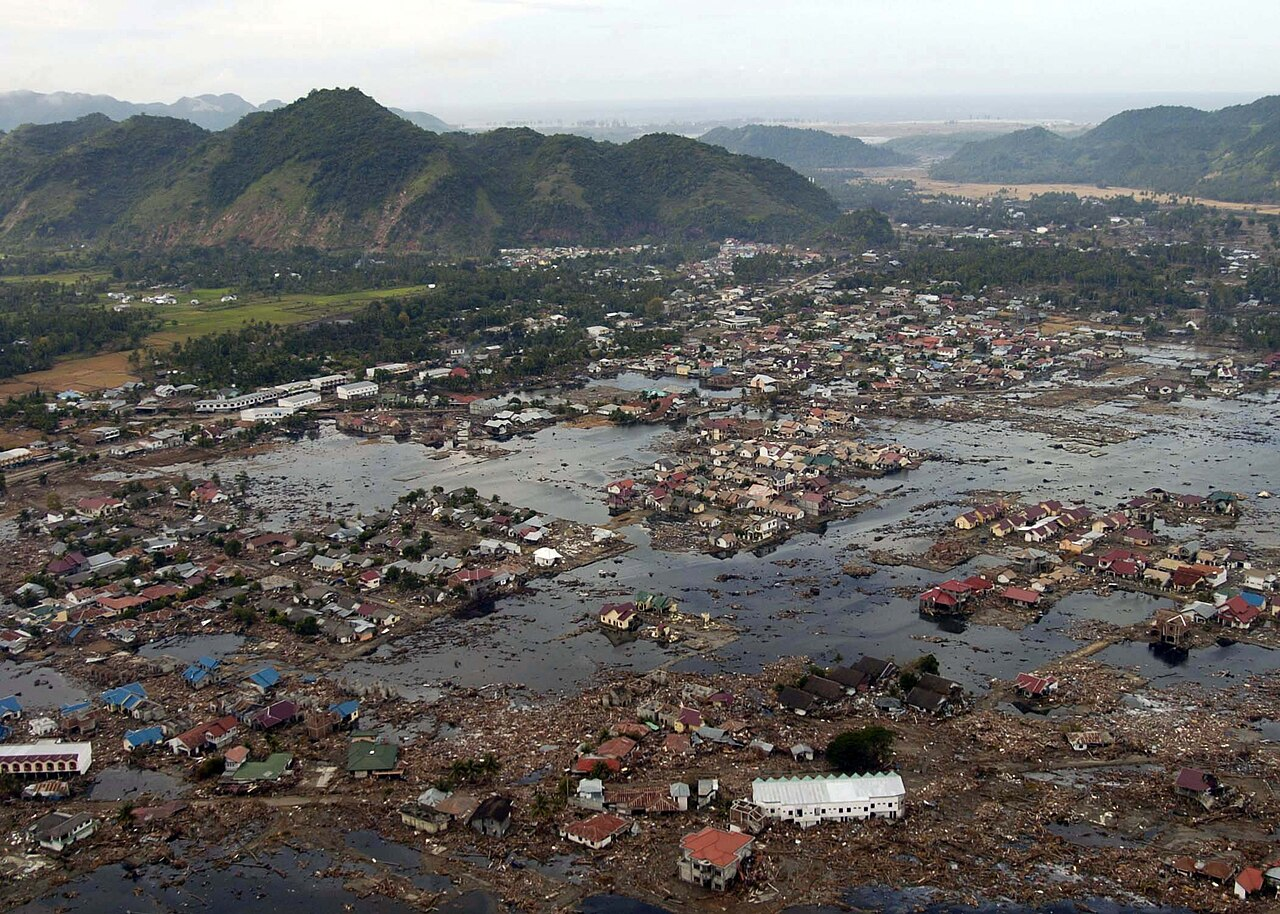
\includegraphics[width=0.78\linewidth]{images/book1/g7-tsunami-village.jpg}

{\small 2004 年 12 月 26 日\omterm{def:g7:earthquakes:tsunami}{海啸}发生一周后，苏门答腊\omterm{def:g1:landscapes-around-us:water}{海岸}附近的一座村庄。
美国海军照片，Philip~A. McDaniel 摄，
公有领域，经由维基共享资源。}
% ledger: commons:tsunami-village
\label{fig:g7:earthquakes:tsunami-village}
\end{omfigure}

\omterm{def:g3:stones-pebbles-sand:rock}{岩石}是如何破裂的？科学家如何在几分钟内找到\omterm{def:g4:volcanoes-earthquakes-first-look:earthquake}{地震}的
发生位置并判断其大小？为什么数小时后，海水会在
无人察觉震动的\omterm{def:g1:landscapes-around-us:water}{海岸}上涨起来？

\begin{recall}
\emph{\omterm{def:g4:volcanoes-earthquakes-first-look:earthquake}{地震}}是地面的突然震动，由
地下深处\omterm{def:g3:stones-pebbles-sand:rock}{岩石}的破裂与错动所引起
（见\cref{ch:g4:volcanoes-earthquakes-first-look}）。地球的外壳由板块构成，
92~\% 的大\omterm{def:g4:volcanoes-earthquakes-first-look:earthquake}{地震}发生在距\omterm{def:g7:plate-tectonics:plate-boundary}{板块边界}
不足 \qty{300}{km} 的范围内（见\cref{ch:g7:plate-tectonics}）。
\omterm{def:g4:volcanoes-earthquakes-first-look:earthquake}{地震}发生时，\omterm{def:g4:volcanoes-earthquakes-first-look:earthquake}{地震}波穿过整个地球的\omterm{def:g3:stones-pebbles-sand:rock}{岩石}，
其中较快的一类是 P~波，较慢的一类是 S~波；通过
比较它们的到达时间，科学家发现了\omterm{def:g6:inside-the-earth:layers}{地核}
（见\cref{ch:g6:inside-the-earth}）。
\end{recall}

\section{岩石的破裂}

板块每年只移动几厘米，但它们的边缘十分粗糙：它们
相互粘连，而板块其余部分仍在运动。边缘附近的\omterm{def:g3:stones-pebbles-sand:rock}{岩石}
会轻微弯曲，如同两端受推的尺子，并储存
能量。当推力最终克服摩擦力，\omterm{def:g3:stones-pebbles-sand:rock}{岩石}
一下子松脱并滑动：这种突然的滑动就是\omterm{def:g4:volcanoes-earthquakes-first-look:earthquake}{地震}。
% ledger: usgs:eq-basics

\begin{definition}[断层]\label{def:g7:earthquakes:fault}
\emph{断层}\index{断层}是\omterm{def:g3:stones-pebbles-sand:rock}{岩石}中的破裂面，破裂面两侧的
两块岩体曾发生相对位移。\omterm{def:g4:volcanoes-earthquakes-first-look:earthquake}{地震}时，两块岩体
沿断层突然滑动；断层越大、滑动越大，
\omterm{def:g4:volcanoes-earthquakes-first-look:earthquake}{地震}也就越大。
\end{definition}

\omterm{def:g7:plate-tectonics:plate-boundary}{板块边界}由许多\omterm{def:g7:earthquakes:fault}{断层}组成，世界上大多数
\omterm{def:g4:volcanoes-earthquakes-first-look:earthquake}{地震}都发生在这些\omterm{def:g7:earthquakes:fault}{断层}上。但\omterm{def:g7:earthquakes:fault}{断层}也存在于板块内部，
其中一些也会破裂。大\omterm{def:g7:earthquakes:fault}{断层}在近地表处破裂时，
滑动可以在地面上看到：田地里出现台阶，道路被截断，
篱笆或一排树木被横向错开。
% ledger: usgs:eq-basics

\begin{omfigure}
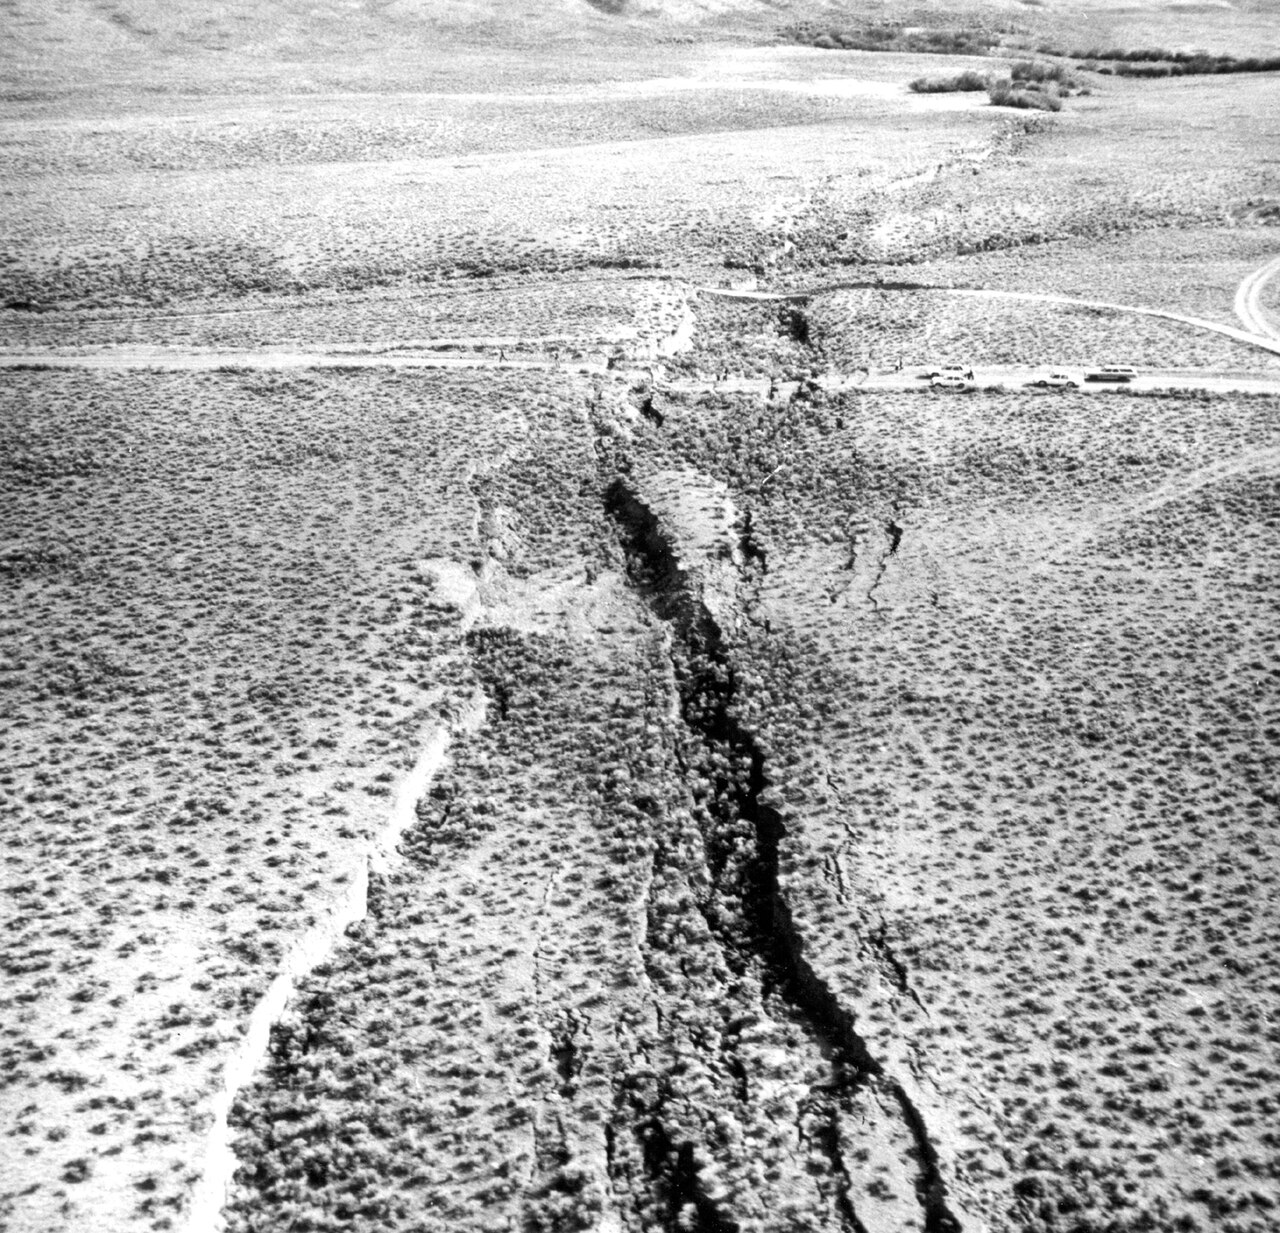
\includegraphics[width=0.62\linewidth]{images/book1/g7-borah-scarp.jpg}

{\small 1983 年博拉峰\omterm{def:g4:volcanoes-earthquakes-first-look:earthquake}{地震}在地面上留下的台阶，地点
位于美国爱达荷州，从空中俯瞰：沿\omterm{def:g7:earthquakes:fault}{断层}，一侧
相对另一侧下降，台阶在
画面上方穿过道路。照片：R.~E. 华莱士，U.S. Geological Survey（公有领域，
经由维基共享资源）。}
% ledger: commons:borah-scarp
\label{fig:g7:earthquakes:borah}
\end{omfigure}

\begin{definition}[震源与震中]\label{def:g7:earthquakes:focus}
\omterm{def:g4:volcanoes-earthquakes-first-look:earthquake}{地震}的\emph{震源}\index{震源}是地下的
\omterm{def:g7:earthquakes:fault}{断层}上滑动开始的位置。\emph{震中}\index{震中}是
地表上正对震源的那一点。
\end{definition}

\omterm{def:g7:earthquakes:focus}{震源}通常位于地下几千米至几十千米深处。在
1976 年至 2025 年间记录到的 7\,031 次 6 级及以上\omterm{def:g4:volcanoes-earthquakes-first-look:earthquake}{地震}中，
5\,561 次——79~\%——\omterm{def:g7:earthquakes:focus}{震源}位于地下不足 \qty{70}{km} 处。
但有 483 次起始于地下超过 \qty{300}{km} 处，最深的
达 \qty{688}{km}。这些深源\omterm{def:g4:volcanoes-earthquakes-first-look:earthquake}{地震}发生在一个板块
俯冲至另一板块之下的地方，位于下沉板块内部。
% ledger: data:usgs-comcat (figdata/grade-7/quake_counts.py, part depth)

大\omterm{def:g4:volcanoes-earthquakes-first-look:earthquake}{地震}很少单独发生，之后常常会有较小的
\omterm{def:g4:volcanoes-earthquakes-first-look:earthquake}{地震}在同一地点相继发生，即\emph{余震}，持续数周、数月甚至
数年。有时较小的\omterm{def:g4:volcanoes-earthquakes-first-look:earthquake}{地震}会先于大\omterm{def:g4:volcanoes-earthquakes-first-look:earthquake}{地震}发生，但在大\omterm{def:g4:volcanoes-earthquakes-first-look:earthquake}{地震}
发生之前无法断定它们是预警。科学家无法
预测\omterm{def:g4:volcanoes-earthquakes-first-look:earthquake}{地震}，只能指出哪些\omterm{def:g7:earthquakes:fault}{断层}将来某一天会再次破裂，
并帮助人们做好准备。
% ledger: usgs:eq-basics, usgs:seismograph

\begin{omfigure}
\begin{tikzpicture}[font=\small, x=1cm, y=1cm]
  % a block of crust seen in perspective: front face and top face
  \def\dx{2.2}\def\dy{1.3}
  % top surface: two blocks separated by the fault trace
  \fill[green!12] (0,0) -- (4.6,0) -- (4.6+\dx,\dy) -- (\dx,\dy) -- cycle;
  \fill[green!18] (4.6,0) -- (9,0) -- (9+\dx,\dy) -- (4.6+\dx,\dy) -- cycle;
  % front face
  \fill[brown!30] (0,0) -- (4.6,0) -- (3.4,-4) -- (0,-4) -- cycle;
  \fill[brown!40] (4.6,0) -- (9,0) -- (9,-4) -- (3.4,-4) -- cycle;
  % right face
  \fill[brown!22] (9,0) -- (9+\dx,\dy) -- (9+\dx,\dy-4) -- (9,-4) -- cycle;
  % fault plane on the front face and trace on top
  \draw[very thick, red!70!black] (4.6,0) -- (3.4,-4);
  \draw[very thick, red!70!black] (4.6,0) -- (4.6+\dx,\dy);
  % slip arrows
  \draw[-{Stealth[length=2.5mm]}, thick] (2.6,-0.35) -- (1.6,-0.35);
  \draw[-{Stealth[length=2.5mm]}, thick] (6.4,-0.35) -- (7.4,-0.35);
  \node[font=\footnotesize, anchor=south] at (2.1,-0.3) {岩块 1};
  \node[font=\footnotesize, anchor=south] at (6.9,-0.3) {岩块 2};
  % focus and waves
  \coordinate (F) at (3.95,-2.4);
  \foreach \r in {0.5,1.0,1.5,2.0}
    \draw[blue!60, dashed] (F) circle (\r);
  \fill[red!80!black] (F) circle (0.13);
  % epicentre: on the surface, straight above the focus (front edge of the top face)
  \coordinate (E) at (3.95,0);
  \draw[black!60, densely dotted, thick] (F) -- (E);
  \node[star, star points=5, star point ratio=2.4, fill=orange, draw=black, inner sep=1.4pt] at (E) {};
  % labels
  \node[anchor=west] at (9.5,-2.3) {震源};
  \draw[black!60] (9.45,-2.3) -- (4.1,-2.4);
  \node[anchor=south west] at (4.9,1.9) {震中};
  \draw[black!60] (4.95,1.95) -- (4.05,0.12);
  \node[anchor=south, red!70!black] at (6.8,1.3) {断层};
  \node[anchor=east, blue!60!black, align=right] at (-0.15,-2.6) {地震波向 \\四面八方传播};
  \draw[blue!60, -{Stealth}] (-0.1,-2.6) -- (1.9,-2.5);
\end{tikzpicture}

{\small \omterm{def:g7:earthquakes:fault}{断层}、\omterm{def:g7:earthquakes:focus}{震源}和\omterm{def:g7:earthquakes:focus}{震中}示意图（非按比例绘制）。
两侧岩块沿\omterm{def:g7:earthquakes:fault}{断层}（红色）相对错动；错动始于
\omterm{def:g7:earthquakes:focus}{震源}，\omterm{def:g4:volcanoes-earthquakes-first-look:earthquake}{地震}波从\omterm{def:g7:earthquakes:focus}{震源}向四面八方传播，如同
池塘中的涟漪。\omterm{def:g7:earthquakes:focus}{震中}（星形）位于地表，
恰在\omterm{def:g7:earthquakes:focus}{震源}正上方。}
% ledger: usgs:eq-basics
\label{fig:g7:earthquakes:fault}
\end{omfigure}


\section{记录地震}

\begin{definition}[地震仪与地震图]\label{def:g7:earthquakes:seismometer}
\emph{地震仪}\index{地震仪}是一种记录
地面震动的仪器。它的记录是一条随时间变化的曲线，称为
\emph{地震图}\index{地震图}。
\end{definition}

\omterm{def:g7:earthquakes:seismometer}{地震仪}的原理很简单。仪器的框架牢牢固定在
地面上，一个重物用弹簧悬挂在框架上。地面震动时，
框架随之震动，但仅由弹簧吊着的重物
几乎保持静止。仪器记录的是框架相对于
静止重物的运动，也就是地面的运动。下
图中，固定在重物上的笔在绕在
转筒上的纸上画出记录。
% ledger: usgs:seismograph

\begin{omfigure}
\begin{tikzpicture}[font=\small, x=1cm, y=1cm]
  \begin{scope}
    % ground
    \fill[brown!30] (-0.6,-0.6) rectangle (5.0,0);
    \draw[decorate, decoration={snake, amplitude=1.2pt, segment length=6pt}, brown!70!black, thick]
      (-0.6,0) -- (5.0,0);
    % frame
    \fill[black!55] (0,0) rectangle (0.25,3.2);
    \fill[black!55] (0,3.0) rectangle (2.4,3.25);
    % spring and weight
    \draw[decorate, decoration={coil, aspect=0.5, segment length=3pt, amplitude=4pt}, thick]
      (2.1,3.0) -- (2.1,2.1);
    \fill[black!80] (1.7,1.45) rectangle (2.5,2.1);
    \node[white, font=\scriptsize] at (2.1,1.78) {质量};
    % pen arm and drum
    \draw[thick] (2.5,1.75) -- (3.45,1.75);
    \fill (3.45,1.75) circle (0.05);
    \draw[thick, fill=white] (3.95,1.75) circle (0.5);
    \draw[thick] (3.95,1.25) -- (3.95,0);
    \draw[-{Stealth}, black!60] (4.55,2.2) arc (40:-40:0.7);
    % labels
    \node[anchor=east, align=right, font=\footnotesize] at (-0.1,2.3) {框架固定 \\在地面上};
    \node[anchor=west, font=\footnotesize] at (2.6,2.65) {弹簧};
    \draw[black!60] (2.55,2.65) -- (2.25,2.6);
    \node[anchor=north, align=center, font=\footnotesize] at (2.1,1.35) {重物：\\保持静止};
    \node[anchor=west, align=left, font=\footnotesize] at (4.7,1.05) {转筒 \\及其上的纸};
    \node[anchor=north, font=\footnotesize] at (2.2,-0.65) {地面震动};
  \end{scope}
  \begin{scope}[xshift=7.2cm, yshift=0.4cm]
    \begin{axis}[width=7.6cm, height=4.2cm, xmin=0, xmax=60, ymin=-1.1, ymax=1.1,
        axis x line=bottom, axis y line=none, xlabel={时间（秒）},
        tick label style={font=\scriptsize}, label style={font=\footnotesize}, clip=false]
      \addplot[black, line width=0.4pt] table[x=t, y=v] {figdata/out/grade-7-epicentre-m-trace.dat};
      \draw[blue!70!black, -{Stealth[length=2mm]}] (axis cs:10,1.45) -- (axis cs:10,0.45);
      \node[blue!70!black, font=\scriptsize, anchor=south east] at (axis cs:10.5,1.45) {较快的波先到达};
      \draw[red!70!black, -{Stealth[length=2mm]}] (axis cs:20,1.45) -- (axis cs:20,1.05);
      \node[red!70!black, font=\scriptsize, anchor=south west] at (axis cs:19.5,1.45) {较慢的波后到达};
      \draw[{Stealth[length=2mm]}-{Stealth[length=2mm]}] (axis cs:10,-0.75) -- (axis cs:20,-0.75);
      \node[font=\scriptsize, anchor=east] at (axis cs:9,-0.75) {延迟：10 秒};
    \end{axis}
  \end{scope}
\end{tikzpicture}

{\small 左：\omterm{def:g7:earthquakes:seismometer}{地震仪}的原理（示意图）。右：为本书绘制的
\omterm{def:g7:earthquakes:seismometer}{地震图}（非实际记录）：曲线先平静，
随后较快的波到达，十秒之后，较慢而
较大的波到达。}
% ledger: usgs:seismograph (trace drawn by figdata/grade-7/epicentre.py, part m-trace)
\label{fig:g7:earthquakes:seismometer}
\end{omfigure}

\subsection*{地震离我们有多远？}

\omterm{def:g7:earthquakes:seismometer}{地震图}提供的信息不止“地面震动了”。较快的波总是
先到达，较慢的波随后到达。靠近\omterm{def:g7:earthquakes:focus}{震源}时，两者
几乎同时到达；远离\omterm{def:g7:earthquakes:focus}{震源}时，较慢的波越落越远，
就像远处打雷时，闪电先到而雷声
滞后得越久，间隔越长。因此，两次到达的时间差
就能说明\omterm{def:g4:volcanoes-earthquakes-first-look:earthquake}{地震}的距离。
% ledger: usgs:seismograph

每秒的延迟对应多少千米？这取决于两种波的速度
在所经过\omterm{def:g3:stones-pebbles-sand:rock}{岩石}中的速度。采用参考
地球参考模型（见\cref{ch:g6:inside-the-earth}）的速度，每秒延迟
对应上\omterm{def:g6:inside-the-earth:layers}{地壳}约 \qty{7}{km}，下
\omterm{def:g6:inside-the-earth:layers}{地壳}约 \qty{9}{km}。本章练习中，我们取
\qty{8}{km}作为每秒的整数值。
% ledger: data:prem (computed in figdata/grade-7/epicentre.py, part rule)

\begin{method}[用三个台站确定震中]\label{met:g7:earthquakes:three-circles}
\begin{enumerate}
  \item 在每个台站的\omterm{def:g7:earthquakes:seismometer}{地震图}上，读出较快的波与
        较慢的波到达之间的延迟。
  \item 将每个延迟换算为距离（此处：$8 \times$ 延迟
        秒数，单位为千米）。
  \item 在\omterm{def:g2:drawing-to-map:map}{地图}上，以每个台站为圆心画一个圆，半径为其
        距离。\omterm{def:g7:earthquakes:focus}{震中}位于每个圆上的某处。
  \item 有两个圆时，通常有两个可能的点；第三个
        圆只经过其中一个点，该点即为\omterm{def:g7:earthquakes:focus}{震中}。
\end{enumerate}
\end{method}

\begin{example}[三个圆]\label{ex:g7:earthquakes:three-circles}
三个台站记录到同一次\omterm{def:g4:volcanoes-earthquakes-first-look:earthquake}{地震}。台站~M1 的延迟为 \qty{10}{s}，
M2 为 \qty{11.25}{s}，M3 为 \qty{9.75}{s}。对应的距离分别为
$8 \times 10 = \qty{80}{km}$、$8 \times 11.25 = \qty{90}{km}$ 和
$8 \times 9.75 = \qty{78}{km}$。下图所示的三个圆
相交于一点：\omterm{def:g7:earthquakes:focus}{震中}。
% ledger: usgs:seismograph (figdata/grade-7/epicentre.py, parts m-stations and m-circles)
\end{example}

\begin{omfigure}
\begin{tikzpicture}
  \begin{axis}[axis equal image, width=8.2cm, xmin=-150, xmax=170, ymin=-160, ymax=160,
      xtick={-120,-80,...,160}, ytick={-120,-80,...,120}, grid=both, grid style={black!12},
      tick label style={font=\scriptsize}, xlabel={km}, ylabel={km}, label style={font=\footnotesize}]
    \addplot[blue!60!black, line width=0.6pt] table[x=x, y=y] {figdata/out/grade-7-epicentre-m-circles.dat};
    \addplot[only marks, mark=triangle*, mark size=3pt, black, point meta=explicit symbolic]
      table[x=x, y=y, meta=name] {figdata/out/grade-7-epicentre-m-stations.dat};
    \node[black, font=\scriptsize, anchor=north, yshift=-2pt] at (axis cs:-48,64) {M1};
    \node[black, font=\scriptsize, anchor=north, yshift=-2pt] at (axis cs:72,54) {M2};
    \node[black, font=\scriptsize, anchor=north, yshift=-2pt] at (axis cs:30,-72) {M3};
    \node[star, star points=5, star point ratio=2.4, fill=orange, draw=black, inner sep=1.6pt] at (axis cs:0,0) {};
    \draw[black!60] (axis cs:-4,-4) -- (axis cs:-60,-75);
    \node[font=\scriptsize, anchor=north east, inner sep=1pt] at (axis cs:-60,-75) {震中};
  \end{axis}
\end{tikzpicture}

{\small 每个圆都以一个台站（三角形）为圆心，
半径等于该台站到\omterm{def:g7:earthquakes:focus}{震源}的距离。三个圆
只相交于一点，即\omterm{def:g7:earthquakes:focus}{震中}（星形）。}
% ledger: usgs:seismograph (figdata/grade-7/epicentre.py, parts m-stations and m-circles)
\label{fig:g7:earthquakes:three-circles}
\end{omfigure}

\begin{omfigure}
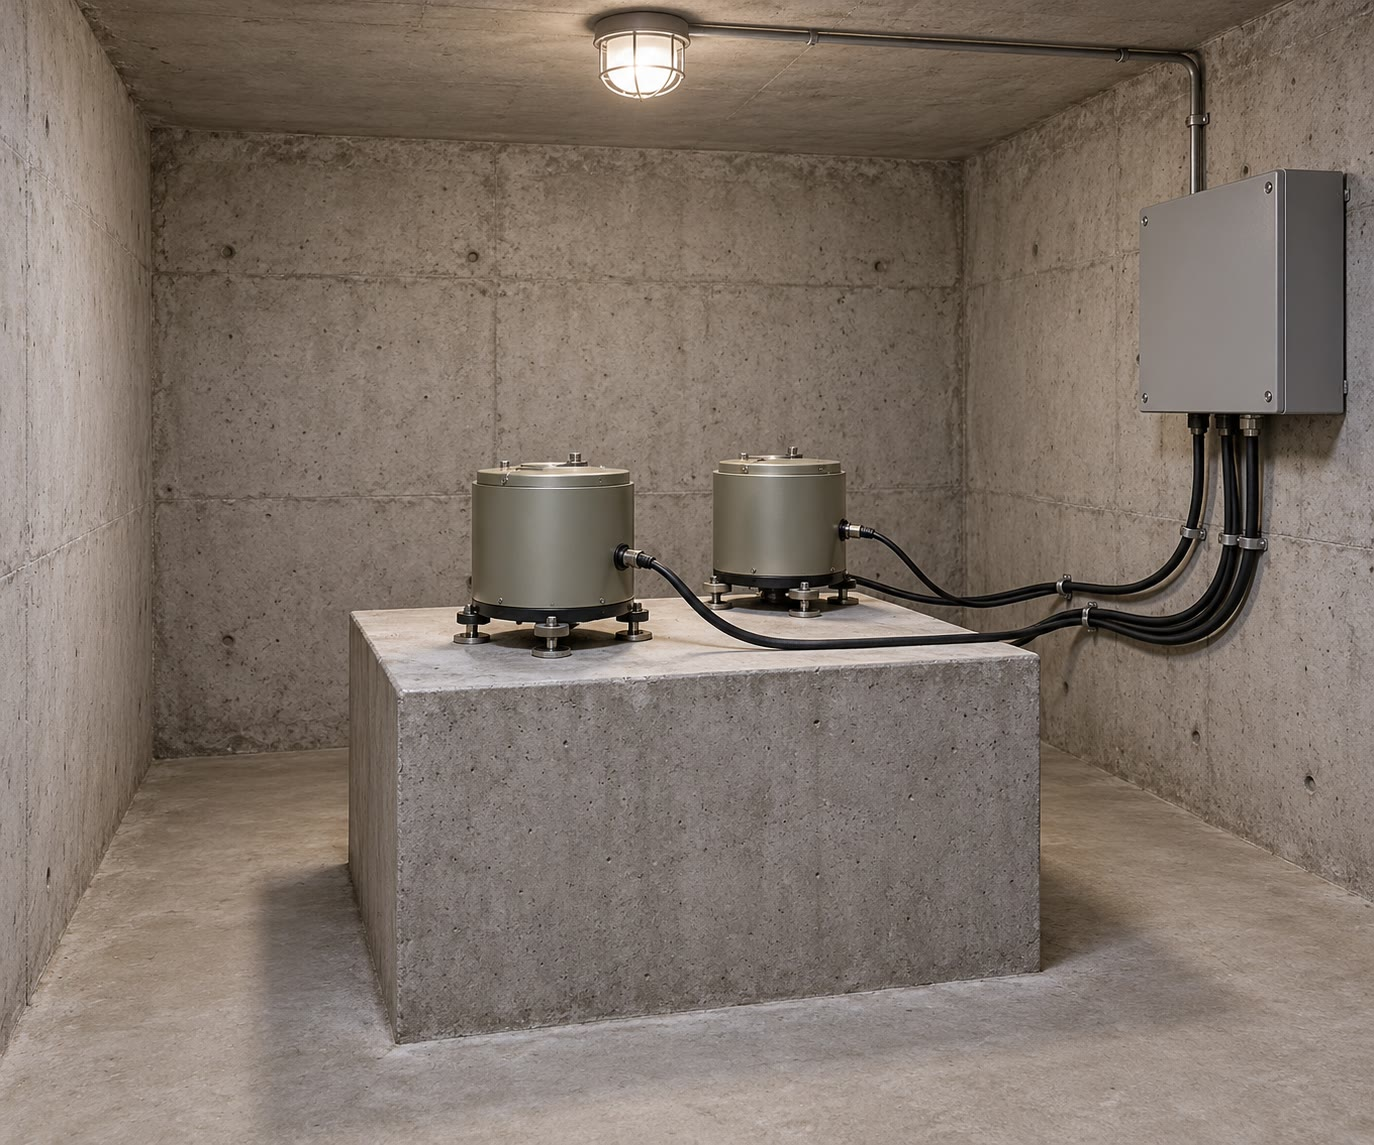
\includegraphics[width=0.58\linewidth]{images/book1/ai/g7-seismometer-vault.jpg}

{\small 安静的地下室里，\omterm{def:g7:earthquakes:seismometer}{地震仪}安放在
直接立于\omterm{def:g3:stones-pebbles-sand:rock}{岩石}上的混凝土墩上，远离道路和机器
（AI 生成的通用场景示意图）。}
\label{fig:g7:earthquakes:vault}
\end{omfigure}

\section{震级有多大？震级与烈度}

两个不同的数用来描述\omterm{def:g4:volcanoes-earthquakes-first-look:earthquake}{地震}，二者常被混淆。

\begin{definition}[震级]\label{def:g7:earthquakes:magnitude}
\omterm{def:g4:volcanoes-earthquakes-first-look:earthquake}{地震}的\emph{震级}\index{震级}衡量\omterm{def:g4:volcanoes-earthquakes-first-look:earthquake}{地震}的大小，
即在\omterm{def:g7:earthquakes:focus}{震源}释放的能量。它由\omterm{def:g7:earthquakes:seismometer}{地震图}计算得出。
每次\omterm{def:g4:volcanoes-earthquakes-first-look:earthquake}{地震}只有一个震级，写成一位小数，例如
6.3 或 9.1。
\end{definition}

\begin{definition}[烈度]\label{def:g7:earthquakes:intensity}
\omterm{def:g4:volcanoes-earthquakes-first-look:earthquake}{地震}在某地的\emph{烈度}\index{烈度}描述
该处地面震动的强烈程度，依据人们的感受和所见的破坏情况确定。
它用罗马数字表示，从 I（无感）到 XII
（完全毁坏）。一次\omterm{def:g4:volcanoes-earthquakes-first-look:earthquake}{地震}有许多烈度，
各地的烈度各不相同。
\end{definition}

\omterm{def:g7:earthquakes:magnitude}{震级}的标度增长很快。\omterm{def:g7:earthquakes:magnitude}{震级}每增加 1，
\omterm{def:g7:earthquakes:seismometer}{地震图}上的波约大 10~倍，释放的能量约多 32~倍。
\omterm{def:g7:earthquakes:magnitude}{震级}为 8 的\omterm{def:g4:volcanoes-earthquakes-first-look:earthquake}{地震}释放的能量约为
\omterm{def:g7:earthquakes:magnitude}{震级}为 6 的\omterm{def:g4:volcanoes-earthquakes-first-look:earthquake}{地震}的 $32 \times 32 \approx 1000$ 倍。
% ledger: usgs:mag-energy

\begin{method}[比较两次地震的震级]\label{met:g7:earthquakes:magnitudes}
要比较两次\omterm{def:g4:volcanoes-earthquakes-first-look:earthquake}{地震}的能量，数出它们\omterm{def:g7:earthquakes:magnitude}{震级}之间相差的整数级数，
每差一级乘以一次 32：差 1 级，为 32~倍；
差 2 级，约为 1000~倍；差 3 级，约为 32\,000~倍。
\end{method}

\begin{example}[震级 9 与震级 7]\label{ex:g7:earthquakes:nine-seven}
2004 年苏门答腊近海的\omterm{def:g4:volcanoes-earthquakes-first-look:earthquake}{地震}\omterm{def:g7:earthquakes:magnitude}{震级}为 9.1。\omterm{def:g7:earthquakes:magnitude}{震级}为 7.1 的\omterm{def:g4:volcanoes-earthquakes-first-look:earthquake}{地震}
比它小两级，释放的能量约相差
$32 \times 32 = 1024$ 倍，即约少 1000~倍。
% ledger: usgs:largest, usgs:mag-energy
\end{example}

有记录以来最大的\omterm{def:g4:volcanoes-earthquakes-first-look:earthquake}{地震}都发生在一块板块俯冲到另一块板块之下的地方：
1960 年 5 月 22 日智利，\omterm{def:g7:earthquakes:magnitude}{震级} 9.5；1964 年阿拉斯加，9.2；
2004 年苏门答腊近海，9.1；2011 年 3 月 11 日日本近海，9.1。
大\omterm{def:g4:volcanoes-earthquakes-first-look:earthquake}{地震}很罕见，\omterm{def:g7:earthquakes:magnitude}{震级}越大越罕见，如图所示：
\omterm{def:g7:earthquakes:magnitude}{震级}每升高一级，次数约减少到原来的十分之一。
% ledger: usgs:largest, data:usgs-comcat

\begin{omfigure}
\begin{tikzpicture}
  \begin{axis}[ybar, width=0.72\linewidth, height=5.4cm, bar width=22pt,
      ymode=log, log origin y=infty, ymin=0.01, ymax=600,
      xtick=data, xticklabels={{6 至 6.9},{7 至 7.9},{8 至 8.9},{9 及以上}},
      xlabel={震级}, ylabel={每年地震次数},
      ytick={0.01,0.1,1,10,100}, yticklabels={0.01,0.1,1,10,100},
      tick label style={font=\scriptsize}, label style={font=\small},
      nodes near coords, point meta=explicit symbolic,
      nodes near coords style={font=\scriptsize}, enlarge x limits=0.18,
      axis x line*=bottom, axis y line*=left]
    \addplot[fill=omThm!45, draw=omThm!80!black] table[x=cls, y=per_year, meta=per_year] {figdata/out/grade-7-quake_counts.dat};
  \end{axis}
\end{tikzpicture}

{\small 1976--2025 年间平均每年的\omterm{def:g4:volcanoes-earthquakes-first-look:earthquake}{地震}次数，按\omterm{def:g7:earthquakes:magnitude}{震级}分列。
纵轴为对数刻度：每条刻线是下一条的十倍。
数据来源：美国地质调查局\omterm{def:g4:volcanoes-earthquakes-first-look:earthquake}{地震}目录（\omterm{def:g7:earthquakes:magnitude}{震级} 6 或以上的\omterm{def:g4:volcanoes-earthquakes-first-look:earthquake}{地震}共
7\,031 次）。}
% ledger: data:usgs-comcat (figdata/grade-7/quake_counts.py, main table)
\label{fig:g7:earthquakes:counts}
\end{omfigure}

\omterm{def:g7:earthquakes:intensity}{烈度}标度没有计算公式，它是一份对各种现象的列举。
表格以简要形式给出。
% ledger: usgs:mmi, usgs:mmi-page

\begin{center}
\small
\begin{tabular}{|c|p{0.8\linewidth}|}
\hline
\textbf{\omterm{def:g7:earthquakes:intensity}{烈度}} & \textbf{人所感知与所见} \\
\hline
I & 几乎无人感觉到 \\
II & 仅少数静止的人能感觉到，尤其是楼上；悬挂的物体可能摆动 \\
III & 室内可感觉到，像有卡车驶过 \\
IV & 室内多数人可感觉到；碗碟、门窗发出响声 \\
V & 几乎所有人都能感觉到，许多人被惊醒；部分碗碟、门窗破碎 \\
VI & 所有人都能感觉到，许多人惊慌；部分重家具移位；有轻微损坏 \\
VII & 建造良好的建筑少有损坏，建造粗劣的建筑损坏严重；部分烟囱折断 \\
VIII & 普通建筑损坏严重，部分局部倒塌；烟囱和墙体倒落 \\
IX & 坚固建筑也遭受严重损坏；建筑偏离地基 \\
X & 多数建筑连同地基毁坏；铁轨弯曲 \\
XI & 几乎没有建筑保存完好；桥梁毁坏 \\
XII & 损毁殆尽；物体被抛向空中 \\
\hline
\end{tabular}
\end{center}
% ledger: usgs:mmi

\omterm{def:g7:earthquakes:intensity}{烈度}通常在\omterm{def:g7:earthquakes:focus}{震中}附近最高，并随
距离增大而减小。但\omterm{def:g7:earthquakes:intensity}{烈度}还取决于地面：坚硬的\omterm{def:g3:stones-pebbles-sand:rock}{岩石}震动最弱，
松软的泥土震动最强。建在松软地面上的城镇，
受到的震动可能比离\omterm{def:g7:earthquakes:focus}{震中}更近、但建在\omterm{def:g3:stones-pebbles-sand:rock}{岩石}上的另一城镇更强烈。
% ledger: usgs:mag-energy

\begin{omfigure}
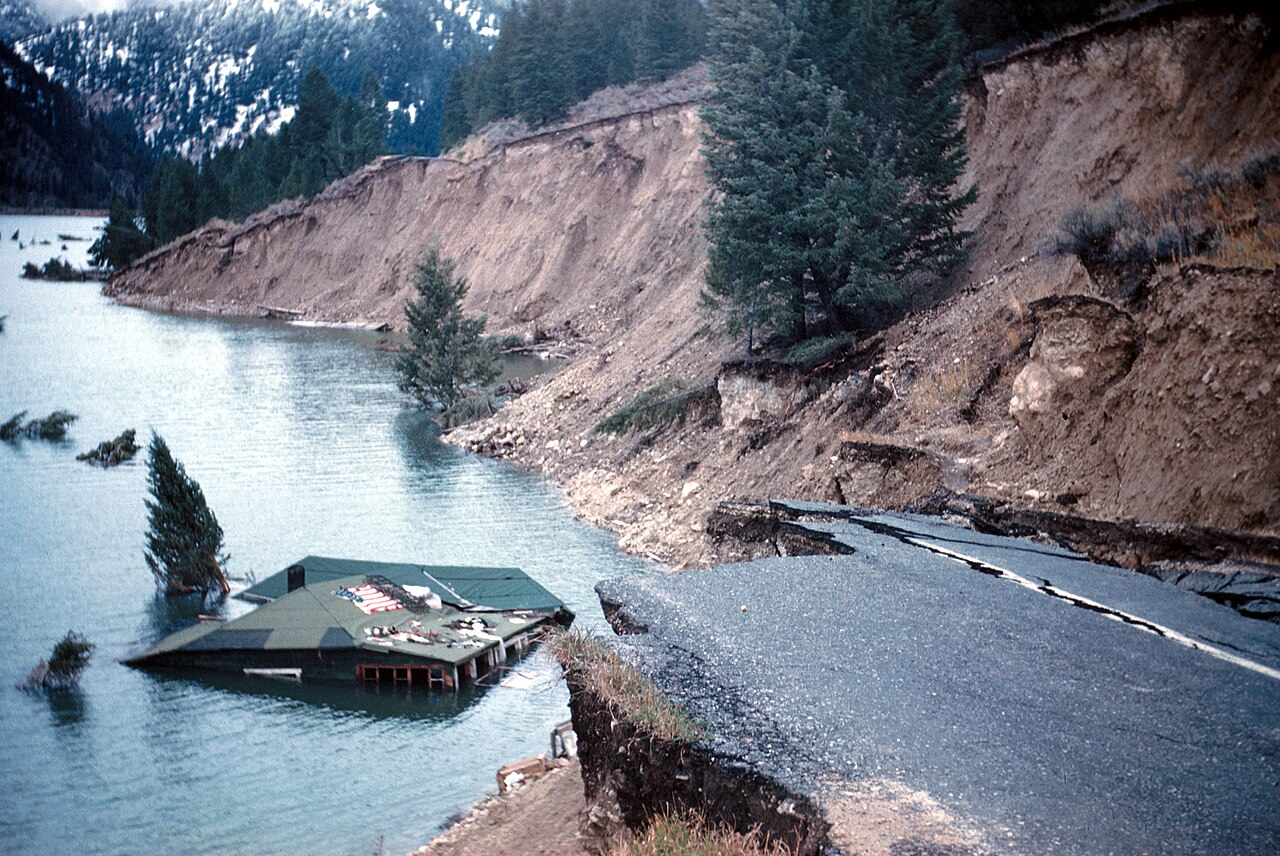
\includegraphics[width=0.6\linewidth]{images/book1/g7-hebgen-road.jpg}

{\small 1959 年 8 月，美国蒙大拿州赫布根湖\omterm{def:g4:volcanoes-earthquakes-first-look:earthquake}{地震}之后：
湖边的公路塌入水中，一座旅馆几乎沉入水下。
这类破坏是高\omterm{def:g7:earthquakes:intensity}{烈度}的标志。
照片：I.~J. Witkind, U.S. Geological Survey（公有领域，经由
维基共享资源）。}
% ledger: commons:hebgen-road, usgs:mmi
\label{fig:g7:earthquakes:hebgen}
\end{omfigure}

\section{海啸}

\begin{definition}[海啸]\label{def:g7:earthquakes:tsunami}
\emph{海啸}\index{海啸}是由海底的突然运动
引发的一系列海浪——通常是海底\omterm{def:g4:volcanoes-earthquakes-first-look:earthquake}{地震}，有时是\omterm{def:g4:volcanoes-earthquakes-first-look:volcano}{火山}\omterm{def:g4:volcanoes-earthquakes-first-look:eruption}{喷发}——
这些海浪可以横穿整个大洋，
淹没沿岸地区。
\end{definition}

当海底的\omterm{def:g7:earthquakes:fault}{断层}破裂时，海底会突然向上或向下运动，
并抬升或降低其上方整个水柱。水以波的形式向外扩散。在深海中，\omterm{def:g7:earthquakes:tsunami}{海啸}
其实并不显眼：波高很少超过一米，船只甚至
察觉不到它从身下经过。但它传播极快，速度超过 \qty{800}{km/h}，
与喷气式飞机相当。当它进入近岸浅水区时，速度减慢
至 30 或 \qty{50}{km/h}——仍快于任何人奔跑——波高随之
增大。多数\omterm{def:g7:earthquakes:tsunami}{海啸}在岸边高度不足 \qty{3}{m}；最大的
可超过 \qty{30}{m}。第一个波未必最大，而且
海浪可能接连到来，持续数小时。
% ledger: nws:tsunami-speed, nws:tsunami-safety

\begin{omfigure}
\begin{tikzpicture}[font=\small, x=1cm, y=1cm]
  % sea floor profile: deep ocean on the left, shelf and coast on the right
  \fill[omSea!35] (0,0) -- (13.2,0) -- (13.2,-0.2) -- (11.4,-0.45) -- (10.2,-1.0) -- (8.8,-2.6) -- (0,-2.6) -- cycle;
  \fill[brown!35] (0,-2.6) -- (8.8,-2.6) -- (10.2,-1.0) -- (11.4,-0.45) -- (13.2,-0.2) -- (13.2,0.5) -- (14.2,1.0) -- (14.2,-3.3) -- (0,-3.3) -- cycle;
  % the broken fault under the sea, at left; one block lifted
  \draw[very thick, red!70!black] (1.9,-3.3) -- (2.3,-2.6);
  \draw[-{Stealth[length=2mm]}, thick] (2.75,-3.1) -- (2.75,-2.75);
  \node[anchor=north west, font=\footnotesize, red!70!black] at (0.1,-3.35) {断层破裂，海底跃升};
  % wave: low and long in the deep ocean, short and tall near the coast
  \draw[blue!70!black, thick] (0,0) .. controls (1.2,0.18) and (2.2,0.18) .. (3.4,0)
     -- (5.0,0) .. controls (5.8,0.12) and (6.6,0.12) .. (7.4,0) -- (10.6,0)
     .. controls (11.0,0.55) and (11.6,0.9) .. (12.1,0) -- (13.2,0);
  \node[align=center, font=\footnotesize] at (2.0,0.85) {深海：约 1 m 高，\\超过 800 km/h};
  \node[align=center, font=\footnotesize] at (11.1,1.55) {近岸：速度减慢 \\（30 至 50 km/h），明显增高};
  \draw[-{Stealth[length=2.5mm]}, thick, blue!70!black] (4.4,0.45) -- (6.4,0.45);
  \node[font=\footnotesize] at (6.0,-1.5) {水深数千米};
  \node[font=\footnotesize] at (12.0,-0.75) {浅水};
\end{tikzpicture}

{\small \omterm{def:g7:earthquakes:tsunami}{海啸}穿越大洋（示意图，非按比例绘制：波高被大幅
夸大）。它在深海上低平而极快，
在近岸浅水区则减速并增高。}
% ledger: nws:tsunami-speed
\label{fig:g7:earthquakes:tsunami}
\end{omfigure}

\begin{example}[从苏门答腊到斯里兰卡]\label{ex:g7:earthquakes:colombo}
斯里兰卡最大城市科伦坡，距离约 \qty{1830}{km}，
即 2004 年\omterm{def:g4:volcanoes-earthquakes-first-look:earthquake}{地震}\omterm{def:g7:earthquakes:focus}{震中}。若以 \qty{800}{km/h} 计，\omterm{def:g7:earthquakes:tsunami}{海啸}
穿越这段距离需要 $1830 \div 800 \approx 2.3$~小时，即约 2~小时
17~分钟。斯里兰卡没有人感觉到\omterm{def:g4:volcanoes-earthquakes-first-look:earthquake}{地震}：\omterm{def:g7:earthquakes:tsunami}{海啸}到来时，
除了海水本身，没有任何预警。
% ledger: nws:tsunami-speed, usgs:largest (distance and time in figdata/grade-7/quake_counts.py, part tsunami)
\end{example}

\begin{remark}[海水发出的预警]\label{rem:g7:earthquakes:natural-warning}
% ledger: nws:tsunami-natural-warning, nws:tsunami-speed, shakeout:dch
在\omterm{def:g1:landscapes-around-us:water}{海岸}，三种迹象可以预示\omterm{def:g7:earthquakes:tsunami}{海啸}：强烈或持续较久的\omterm{def:g4:volcanoes-earthquakes-first-look:earthquake}{地震}；
海水表现反常——突然涨水，或水体远离\omterm{def:g1:landscapes-around-us:water}{海岸}退去，
露出海底，如同极低的退潮；或有来自\omterm{def:g2:water-on-earth:ocean}{海洋}的
巨大轰鸣。\omterm{def:g4:volcanoes-earthquakes-first-look:earthquake}{地震}摇晃期间，要
按所学方法保护自己（趴下、掩护、抓牢）。随后不要等待
官方预警，应立即尽可能向高处或内陆远处转移。
附近\omterm{def:g4:volcanoes-earthquakes-first-look:earthquake}{地震}引发的\omterm{def:g7:earthquakes:tsunami}{海啸}可能在几分钟内到达。
\end{remark}


\section{练习}

\begin{exercise}[$\star$]\label{exo:g7:earthquakes:1}
将下列词语与其含义配对：\omterm{def:g7:earthquakes:fault}{断层}；\omterm{def:g7:earthquakes:focus}{震源}；\omterm{def:g7:earthquakes:focus}{震中}；\omterm{def:g7:earthquakes:seismometer}{地震仪}；
\omterm{def:g7:earthquakes:magnitude}{震级}；\omterm{def:g7:earthquakes:intensity}{烈度}。（a）地下开始发生滑动的位置。（b）
某一地点地面摇晃的强烈程度。（c）\omterm{def:g3:stones-pebbles-sand:rock}{岩石}中的一处断裂，
断裂两侧已发生相对移动。（d）地表上位于
\omterm{def:g7:earthquakes:focus}{震源}正上方的点。（e）\omterm{def:g4:volcanoes-earthquakes-first-look:earthquake}{地震}的大小，每次\omterm{def:g4:volcanoes-earthquakes-first-look:earthquake}{地震}只有一个数值。（f）
记录地面震动的仪器。
\end{exercise}

\begin{exercise}[$\star$]\label{exo:g7:earthquakes:2}
某次\omterm{def:g4:volcanoes-earthquakes-first-look:earthquake}{地震}的\omterm{def:g7:earthquakes:focus}{震源}位于一个村庄正下方 \qty{30}{km} 处。
（a）\omterm{def:g7:earthquakes:focus}{震中}在哪里？（b）村庄距\omterm{def:g7:earthquakes:focus}{震源}多远？
（c）第二个村庄距\omterm{def:g7:earthquakes:focus}{震中} \qty{40}{km}，它的
\omterm{def:g7:earthquakes:intensity}{烈度}通常比第一个村庄更高还是更低？为什么？
\end{exercise}

\begin{exercise}[$\star$]\label{exo:g7:earthquakes:3}
是\omterm{def:g7:earthquakes:magnitude}{震级}还是\omterm{def:g7:earthquakes:intensity}{烈度}？（a）“这次\omterm{def:g4:volcanoes-earthquakes-first-look:earthquake}{地震}测得 6.8。”（b）“在我们
街上，所有碗碟都掉了，一座烟囱也倒塌了。”（c）“镇上为 VI 度，
\omterm{def:g1:landscapes-around-us:landform}{丘陵}上的村庄为 IV 度。”（d）“它释放的能量
是去年那次的 32~倍。”
\end{exercise}

\begin{exercise}[$\star$]\label{exo:g7:earthquakes:4}
判断下列说法是否正确，并改正错误的说法。（a）科学家能提前一周
准确预知\omterm{def:g4:volcanoes-earthquakes-first-look:earthquake}{地震}何时发生。（b）在开阔的\omterm{def:g2:water-on-earth:ocean}{海洋}中，\omterm{def:g7:earthquakes:tsunami}{海啸}是
一堵巨大的水墙。（c）一次\omterm{def:g4:volcanoes-earthquakes-first-look:earthquake}{地震}只有一个\omterm{def:g7:earthquakes:magnitude}{震级}，却有
多个\omterm{def:g7:earthquakes:intensity}{烈度}。（d）大多数大\omterm{def:g4:volcanoes-earthquakes-first-look:earthquake}{地震}发生在\omterm{def:g7:plate-tectonics:plate-boundary}{板块边界}附近。
\end{exercise}

\begin{exercise}[$\star\star$]\label{exo:g7:earthquakes:5}
利用每年\omterm{def:g4:volcanoes-earthquakes-first-look:earthquake}{地震}次数的统计图。（a）每年大约有多少次
\omterm{def:g7:earthquakes:magnitude}{震级}为 6 至 6.9 的\omterm{def:g4:volcanoes-earthquakes-first-look:earthquake}{地震}？\omterm{def:g7:earthquakes:magnitude}{震级}为 7 至 7.9 的呢？（b）第二类
\omterm{def:g4:volcanoes-earthquakes-first-look:earthquake}{地震}次数是第一类的几分之一？（c）将从 7 级起的三根柱子相加，
每年大约有多少次\omterm{def:g7:earthquakes:magnitude}{震级}为 7 级或以上的\omterm{def:g4:volcanoes-earthquakes-first-look:earthquake}{地震}？（d）图表显示，
\omterm{def:g7:earthquakes:magnitude}{震级}为 9 级或以上的\omterm{def:g4:volcanoes-earthquakes-first-look:earthquake}{地震}每年平均 0.04 次。那么
50~年内大约会发生多少次？
\end{exercise}

\begin{exercise}[$\star\star$]\label{exo:g7:earthquakes:6}
利用比较\omterm{def:g7:earthquakes:magnitude}{震级}的方法。（a）\omterm{def:g7:earthquakes:magnitude}{震级}为 7 的\omterm{def:g4:volcanoes-earthquakes-first-look:earthquake}{地震}释放的能量是
\omterm{def:g7:earthquakes:magnitude}{震级}为 6 的\omterm{def:g4:volcanoes-earthquakes-first-look:earthquake}{地震}的多少倍？（b）\omterm{def:g7:earthquakes:magnitude}{震级}为 8 的\omterm{def:g4:volcanoes-earthquakes-first-look:earthquake}{地震}释放的能量，
是\omterm{def:g7:earthquakes:magnitude}{震级}为 6 的\omterm{def:g4:volcanoes-earthquakes-first-look:earthquake}{地震}的多少倍？（c）在相同距离处，
\omterm{def:g7:earthquakes:magnitude}{震级}从 6 增至 8 时，\omterm{def:g7:earthquakes:seismometer}{地震图}上的波形振幅
大了多少倍？
\end{exercise}

\begin{exercise}[$\star\star$]\label{exo:g7:earthquakes:7}
取 \qty{8}{km} 作为快波与慢波之间每延迟一秒对应的距离，
（a）某台站记录到的延迟为 \qty{5}{s}，
\omterm{def:g4:volcanoes-earthquakes-first-look:earthquake}{地震}发生在多远处？（b）另一台站记录到 \qty{25}{s}。（c）某次\omterm{def:g4:volcanoes-earthquakes-first-look:earthquake}{地震}
发生在距某台站 \qty{120}{km} 处，该台站将读到多长的延迟？
（d）为什么仅凭一个台站无法确定\omterm{def:g7:earthquakes:focus}{震中}的位置？
\end{exercise}

\begin{exercise}[$\star\star$]\label{exo:g7:earthquakes:8}
利用\omterm{def:g7:earthquakes:intensity}{烈度}表，给出每份报告对应的\omterm{def:g7:earthquakes:intensity}{烈度}。（a）“几乎所有人都感觉到了，
我们被震醒了，两只玻璃杯碎了。”（b）“只有
在楼上休息的奶奶感觉到了，吊灯晃动了。”（c）“墙体
和烟囱倒塌，好几座房屋部分坍塌。”（d）同一次\omterm{def:g4:volcanoes-earthquakes-first-look:earthquake}{地震}
产生了报告（a）和（c）。请解释这是如何可能的。
\end{exercise}

\begin{exercise}[$\star\star$]\label{exo:g7:earthquakes:9}
在 1976--2025 年间，\omterm{def:g7:earthquakes:magnitude}{震级}为 6 级或以上的 7\,031 次\omterm{def:g4:volcanoes-earthquakes-first-look:earthquake}{地震}中，有 5\,561 次
\omterm{def:g7:earthquakes:focus}{震源}深度小于 \qty{70}{km}。（a）有多少次\omterm{def:g7:earthquakes:focus}{震源}更深？
（b）这一数字占比多少？四舍五入到整数。（c）深源\omterm{def:g4:volcanoes-earthquakes-first-look:earthquake}{地震}
发生在一个板块俯冲到另一板块之下处。请解释为什么它们能
在如此深的地方发生。
\end{exercise}

\begin{exercise}[$\star\star$]\label{exo:g7:earthquakes:10}
马累是马尔代夫的首都，距 2004 年\omterm{def:g4:volcanoes-earthquakes-first-look:earthquake}{地震}的
\omterm{def:g7:earthquakes:focus}{震中}约 \qty{2500}{km}。（a）以 \qty{800}{km/h} 的速度计算，
\omterm{def:g7:earthquakes:tsunami}{海啸}需要多长时间才能到达那里？请以小时和分钟给出。（b）它比
到达科伦坡（2~小时 17~分钟）晚多久？（c）在这样的延迟下，
为什么预警系统可能挽救许多生命？
\end{exercise}

\begin{exercise}[$\star\star\star$]\label{exo:g7:earthquakes:11}
\omterm{def:g7:earthquakes:tsunami}{海啸}以 \qty{800}{km/h} 的速度穿过 \qty{400}{km} 的深海，然后
以 \qty{40}{km/h} 的速度穿过最后 \qty{20}{km} 的浅水区。（a）
深海部分需要多少分钟？（b）浅水部分呢？（c）整个行程
需要多长时间？（d）你的答案中有哪些令人意外的地方？（e）
为什么波浪在减速时会变得更高？
\end{exercise}

\begin{exercise}[$\star\star\star$]\label{exo:g7:earthquakes:12}
（a）\omterm{def:g7:earthquakes:magnitude}{震级}为 9 的\omterm{def:g4:volcanoes-earthquakes-first-look:earthquake}{地震}释放的能量是
\omterm{def:g7:earthquakes:magnitude}{震级}为 6 的\omterm{def:g4:volcanoes-earthquakes-first-look:earthquake}{地震}的多少倍？（b）每年大约发生 127 次\omterm{def:g7:earthquakes:magnitude}{震级}为 6 至 6.9 的\omterm{def:g4:volcanoes-earthquakes-first-look:earthquake}{地震}。
假设其中每一次都释放相当于\omterm{def:g7:earthquakes:magnitude}{震级} 6 的能量，
那么需要多少年的这类\omterm{def:g4:volcanoes-earthquakes-first-look:earthquake}{地震}，才能释放出
一次\omterm{def:g7:earthquakes:magnitude}{震级} 9 \omterm{def:g4:volcanoes-earthquakes-first-look:earthquake}{地震}的能量？（c）这说明最大\omterm{def:g4:volcanoes-earthquakes-first-look:earthquake}{地震}
所携带的能量占比有何特点？
\end{exercise}

\section{问题：地面在哪里摇晃？}

\begin{problem}[{周末问题——三个台站记录到一次海底地震，
在地图上确定了震中，并在海啸到达前
向波特黑尔镇发出了预警}]
\label{pb:g7:earthquakes:1}
% ledger: nws:tsunami-speed, usgs:seismograph, data:prem (figdata/grade-7/epicentre.py)
一次\omterm{def:g4:volcanoes-earthquakes-first-look:earthquake}{地震}发生在一处虚构\omterm{def:g1:landscapes-around-us:water}{海岸}的海底。三个\omterm{def:g7:earthquakes:seismometer}{地震仪}台站
A、B 和 C 位于陆地上；波特黑尔镇位于一座岛屿上（见下图；
每个方格代表 \qty{20}{km}）。在这一地区，
快波与慢波之间每延迟一秒，
对应 \qty{8}{km}。各台站的记录如下：

\begin{center}
\small
\begin{tabular}{|c|c|c|}
\hline
\textbf{台站} & \textbf{快波到达时间} & \textbf{慢波到达时间} \\
\hline
A & 10:15:25 & 10:15:45 \\
B & 10:15:16 & 10:15:29 \\
C & 10:15:19 & 10:15:34 \\
\hline
\end{tabular}
\end{center}

\medskip
\noindent\textbf{第一部分——三个台站。}\par\nopagebreak
\begin{enumerate}[beginpenalty=10000]
  \item 对每个台站，求两次到达之间的延迟，
        单位为秒。
  \item 哪个台站离\omterm{def:g7:earthquakes:focus}{震中}最近？
        不经计算，你如何判断？
  \item 求每个台站到\omterm{def:g7:earthquakes:focus}{震中}的距离。
  \item 仅凭台站 A 的距离，无法确定\omterm{def:g7:earthquakes:focus}{震中}的位置。
        请描述所有与 A 的距离相同的地点。
\end{enumerate}

\begin{center}
\begin{tikzpicture}
  \begin{axis}[axis equal image, width=12cm, xmin=-60, xmax=360, ymin=-200, ymax=260,
      xtick={-60,-40,...,360}, ytick={-200,-180,...,260}, xticklabels={}, yticklabels={},
      major tick length=0pt,
      axis background/.style={fill=omSea!25}, clip mode=individual]
    \addplot[fill=omLithAlluv, draw=black!50, line width=0.4pt] table[x=x, y=y] {figdata/out/grade-7-epicentre-p-west.dat};
    \addplot[fill=omLithAlluv, draw=black!50, line width=0.4pt] table[x=x, y=y] {figdata/out/grade-7-epicentre-p-north.dat};
    \addplot[fill=omLithAlluv, draw=black!50, line width=0.4pt] table[x=x, y=y] {figdata/out/grade-7-epicentre-p-island.dat};
    % the grid over land and sea, drawn before the labels
    \pgfplotsinvokeforeach{-40,-20,...,340}{\draw[black!15] (axis cs:#1,-200) -- (axis cs:#1,260);}
    \pgfplotsinvokeforeach{-180,-160,...,240}{\draw[black!15] (axis cs:-60,#1) -- (axis cs:360,#1);}
    \addplot[only marks, mark=triangle*, mark size=3.2pt, black, point meta=explicit symbolic]
      table[x=x, y=y, meta=name] {figdata/out/grade-7-epicentre-p-stations.dat};
    \node[black, font=\small\bfseries, anchor=south west] at (axis cs:24,-38) {A};
    \node[black, font=\small\bfseries, anchor=south west] at (axis cs:160,186) {B};
    \node[black, font=\small\bfseries, anchor=south west] at (axis cs:0,90) {C};
    \addplot[only marks, mark=square*, mark size=2.4pt, red!70!black, point meta=explicit symbolic]
      table[x=x, y=y, meta=name] {figdata/out/grade-7-epicentre-p-town.dat};
    \node[red!70!black, font=\small, anchor=north east, fill=omSea!25, inner sep=1pt] at (axis cs:264,-102) {黑尔港};
    \draw[-{Stealth[length=2.5mm]}, line width=0.8pt] (axis cs:330,200) -- (axis cs:330,245);
    \node[font=\scriptsize\bfseries, anchor=north] at (axis cs:330,200) {北};
    \node[font=\scriptsize, anchor=west, fill=omLithAlluv, inner sep=1pt] at (axis cs:170,240) {1 方格 = 20 km};
    \fill (axis cs:-60,-200) circle (1.5pt);
    \node[font=\small\bfseries, anchor=north east] at (axis cs:-60,-200) {O};
  \end{axis}
\end{tikzpicture}
\end{center}
% ledger: (invented map: figdata/grade-7/epicentre.py, parts p-west, p-north, p-island, p-stations, p-town)

\medskip
\noindent\textbf{第二部分——确定\omterm{def:g7:earthquakes:focus}{震中}。}\par\nopagebreak
\begin{enumerate}[resume, beginpenalty=10000]
  \item 每方格为 \qty{20}{km}。
        每个圆的半径为多少方格？
  \item 将 O 点置于\omterm{def:g2:drawing-to-map:map}{地图}左下角。台站 C 位于 O 点向东 3~格、
        向北 14.5~格处；由 C 点正东方向走 6~格
        （\qty{120}{km}），到达点~E。在\omterm{def:g2:drawing-to-map:map}{地图}上检验
        E 点也在 A、B 两圆上，它即为\omterm{def:g7:earthquakes:focus}{震中}。
        它在 O 点的东、北方向各多少格？
  \item \omterm{def:g7:earthquakes:focus}{震中}位于陆地还是海底？这有什么意义？
  \item 该\omterm{def:g4:volcanoes-earthquakes-first-look:earthquake}{地震}的\omterm{def:g7:earthquakes:magnitude}{震级}为 7.4。它释放的能量是
        \omterm{def:g7:earthquakes:magnitude}{震级}为 6.4 的\omterm{def:g4:volcanoes-earthquakes-first-look:earthquake}{地震}的多少倍？
\end{enumerate}

\medskip
\noindent\textbf{第三部分——\omterm{def:g7:earthquakes:tsunami}{海啸}抵达\omterm{def:g1:landscapes-around-us:water}{海岸}。}\par\nopagebreak
\begin{enumerate}[resume, beginpenalty=10000]
  \item 在\omterm{def:g2:drawing-to-map:map}{地图}上，黑尔港距\omterm{def:g7:earthquakes:focus}{震中} 12~格，
        这相当于多少千米？
  \item \omterm{def:g7:earthquakes:tsunami}{海啸}以 \qty{800}{km/h} 的速度传播，
        多少分钟能抵达黑尔港？
  \item 确定\omterm{def:g4:volcanoes-earthquakes-first-look:earthquake}{地震}位置并发出预警，耗时 5~分钟，
        自震动开始起算。\omterm{def:g4:volcanoes-earthquakes-first-look:earthquake}{地震}发生后多久，
        预警才能抵达黑尔港？
  \item 黑尔港居民在\omterm{def:g7:earthquakes:tsunami}{海啸}抵达前，还有多少分钟
        可以撤到高地？
\end{enumerate}
\end{problem}
